\chapter{A Dimensional Contextual Semantic Model for music description}
\label{Chap:DCSM}
In the past few decades, the importance of high-level (semantic) description of musical content has progressively grown to the point of becoming a fundamental task in music retrieval applications. In particular, Query By Semantic Description (QBSD) \cite{Turnbull2007,Zanoni2012,Buccoli2013} based on dimensional approaches has gained a great deal of popularity. %In dimensional approaches, terms are represented in a metric space where the distance describes semantic similarity. 
In Section \ref{sec:HLFs:ANEW} we proposed an evolution of the dimensional Valence-Arousal semantic model for emotional-related descriptors, while in Chapter \ref{Chap:Violin} we explored timbral descriptions for violin instruments. %The interest in dimensional models has recently grown a great deal, as they define a semantic relation between concepts through "graded" descriptions. In Section \ref{HLFs:semantic}

In general, the mood and the timbre of a song are just two of the several aspects of music. In order to obtain a more extensive formalization of the semantic domain, a dimensional semantic model needs to take into consideration a wide range of aspects. The approaches to achieve this can be grouped in two broad categories: the definition of a generic dimensional model for all the descriptors in different aspects; and the definition of a specific model for each musical aspect.

The former approach has been implemented by taking advantage of user tagging \cite{lamere2009, Barrington2009}, where the semantic relation between terms is inferred from the co-occurrence of descriptors \cite{Levy2007, Sordo2010, Laurier2009} through Latent Semantic Analysis (LSA) \cite{Deerwester1990}, as discussed in Section \ref{sec:HLFs:LSA}. This approach has proved to be quite effective, though it tends to represent all the terms, therefore all the different aspects, in a single semantic space. 

The latter approach has been followed in our previous work \cite{Buccoli2013}, where we proposed a semantic model with emotional-related descriptors, represented by means of the VA space, and with non emotional-related descriptors, represented as a set of bipolar descriptors. In the proposed approach, each aspect (emotional and non-emotional) corresponds to a semantic model with its own exclusive set of descriptors, i.e., each descriptor can describe only one aspect. The overall approach proposed in \cite{Buccoli2013} was named \textit{JANAS} after a traditional myth from Sardinia, Italy. In the following, we will also use the name JANAS to refer to the approach from \cite{Buccoli2013}.  

The LSA and JANAS, however, do not account for the fact that the meaning of terms in natural language could change depending on the context (\textit{polysemy}), such as the term \textit{soft}, which could describe timbral and emotional proprieties.

Ignoring polysemy introduces bias in the music description. For example, let us consider the terms \textit{Anxious} and \textit{Hard}, who are close together in the VA space, and they are likely to be placed close to each other by a LSA-based system, since they are frequently used together. In the VA space, moreover, the two terms are far from the term \textit{Soft}. However, the descriptors \textit{Hard} and \textit{Soft} are often used for addressing timbral properties, as shown in Chapter \ref{Chap:Violin}. Therefore, this could be misleading, as \textit{Anxious} songs could be thought of as \textit{Hard} as well as \textit{Soft}, which is a scenario not expected by LSA. 

The issues raised by polysemy was present in \cite{Buccoli2013} as well, since it modeled the music descriptors as belonging to only one aspect. This also led to some issue in the modeling step, since among the bipolar descriptors there were \textit{Soft} and \textit{Hard}, which also have a semantics for the context of mood.


 \begin{figure}[tbp]
    \begin{center}
      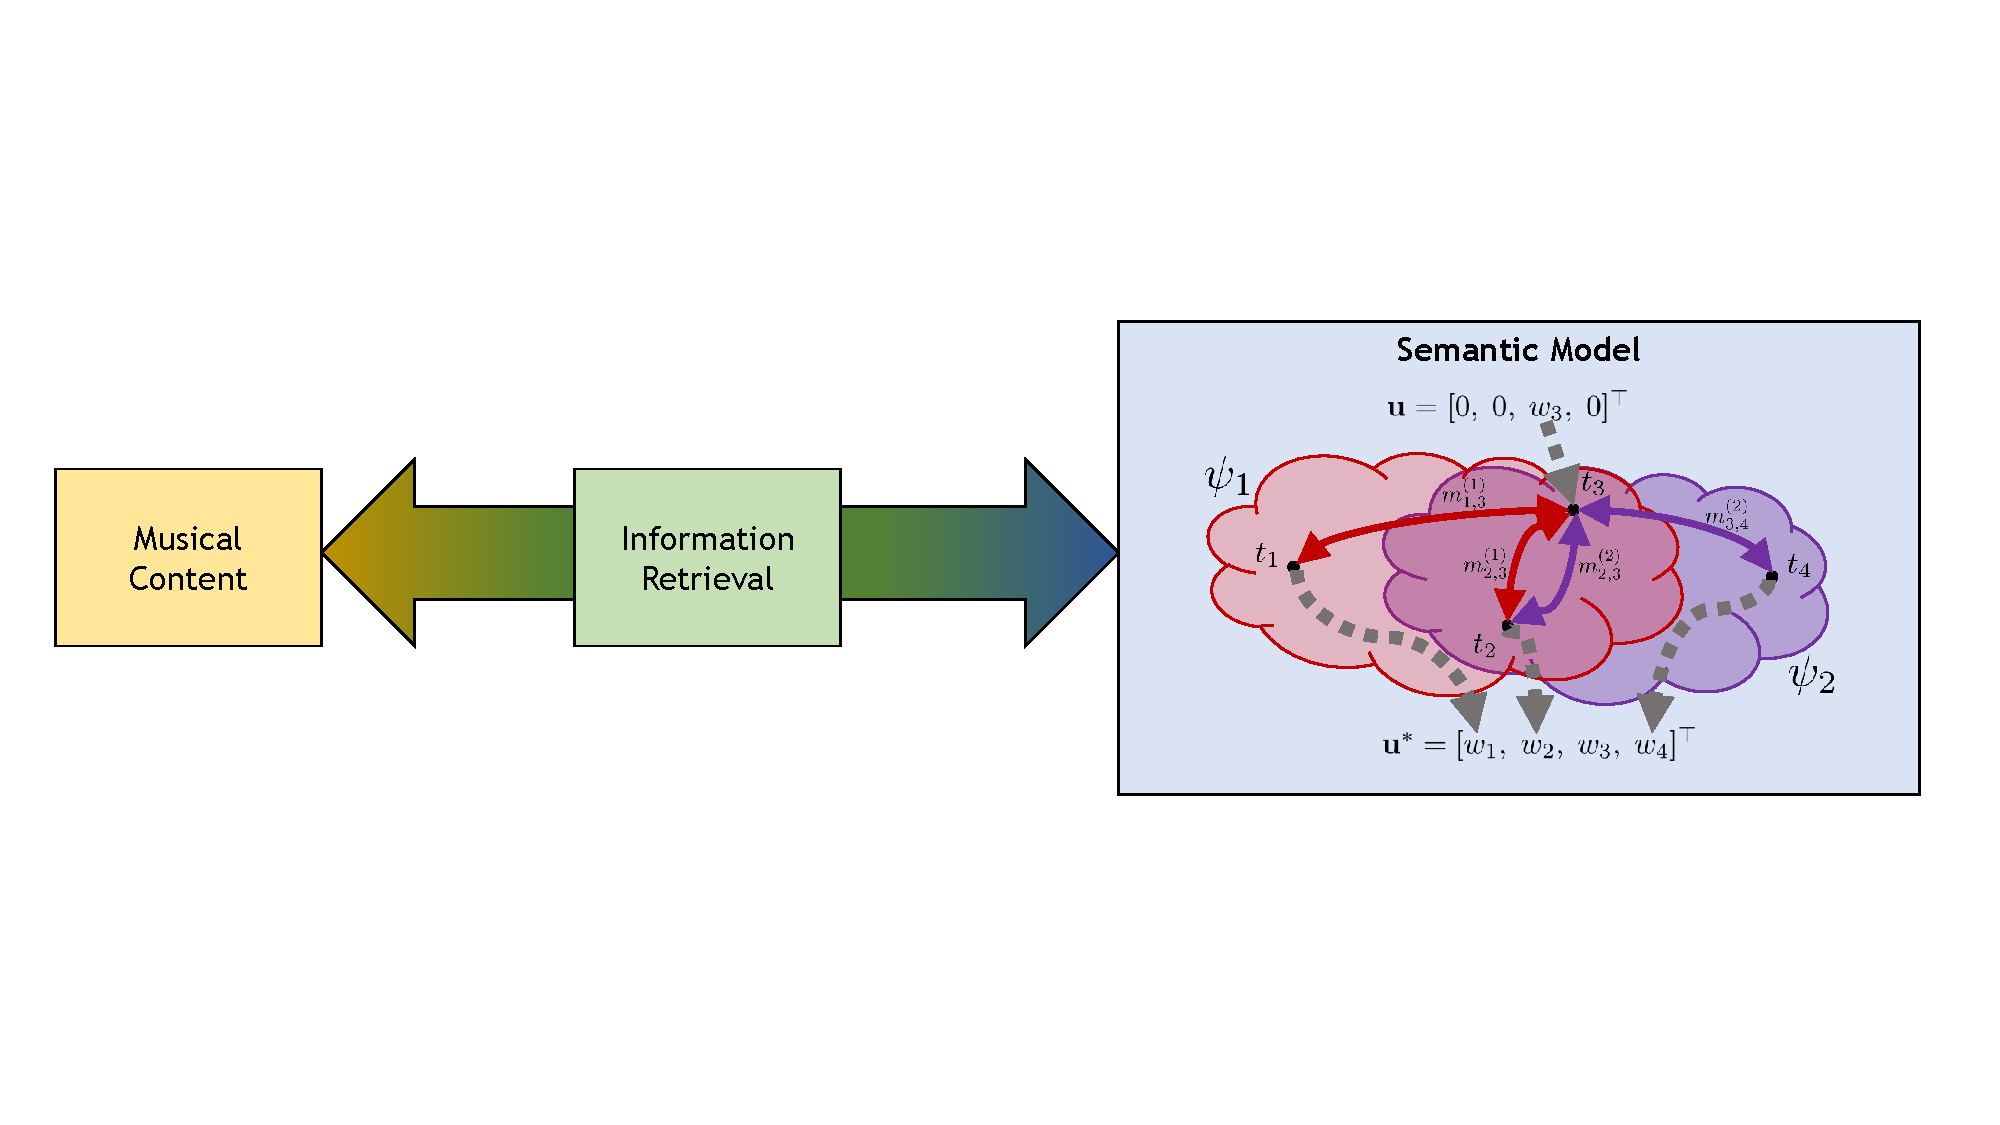
\includegraphics[trim=0.8cm 5.6cm 0.8cm 5.2cm,clip=true,width=\textwidth]{img/DCSM/musical}
	%\psfig{file=im/ML/logopm.jpg,width=3.5cm}
    \end{center}
  \caption{An overview of the application of the paradigm in the proposed application scenario}
  \label{fig:DCSM:scheme}
  \end{figure}


Approaches based on non-negative matrix factorization (NMF) have been proven to be effective for solving polysemy issues \cite{lee1999}. However, they still have not been applied to scenarios where polysemy involves nuances of meaning in the same broad topic (e.g. music description).

In this Chapter, we propose a music description paradigm based on a Dimensional Contextual Semantic Model (DCSM). High-level descriptors are grouped into contexts that represent different aspects of music and each term can belong to several contexts, in order to account for polysemy. Within the contexts, the semantic relationship between descriptors is modeled by means of a graded semantic similarity that ranges from antonymy, to neutrality, to synonymy. 

This problem involves a high degree of complexity from all its components. The semantic model helps the formalization of the semantic domain by directly addressing the ambiguity of the natural language. We use the same semantic model to describe the musical items from the signal domain, in order to have a direct high-level description. Moreover, the set of rules for the definition of the semantic model also acts as the linking function between the semantic description of the signal domain and the possible query from the semantic domain.

%This approach can address the bias in music description and the misleading interpretation of the user query by exploiting semantic similarities and context information.
In order to collect \textit{a-priori} information about contexts and similarity among descriptors, we conducted a two-step online surveys. We evaluate the model in a real-case scenario, by developing a semantic music search engine, which is able to process a natural language query and map the request into the semantic models, hence retrieving the songs that best match the request. We develop three different prototypes of the search engine, one to test the DCSM and the other two as a comparison, using a LSA-based and the JANAS-based semantic models. This study was presented at the International Conference on Acoustics, Speech and Signal Processing (ICASSP) \cite{buccoli2015dimensional}.


In Figure \ref{fig:DCSM:scheme} we summarize our contribution in the described application scenario. The proposed semantic model is used as the framework for the linking function modeled as an information retrieval system, that is able to retrieve the musical content.
In the following Sections we describe the details of the semantic model. We also provide an overview of the implementation of the prototype of the search engine. We describe the experimental setup and we discuss the performance achieved by the DCSM, which is evaluated with a subjective test.



 \section{The semantic model}
\label{sec:DCSMoverview}
In this Section we define the DCSM and we explain how it models the polysemy. We then examine how the musical items and user queries are described in the DCSM and how they exploit the DCSM to overcome annotation or query ambiguity.


\begin{figure}[tbp]
        \centering
         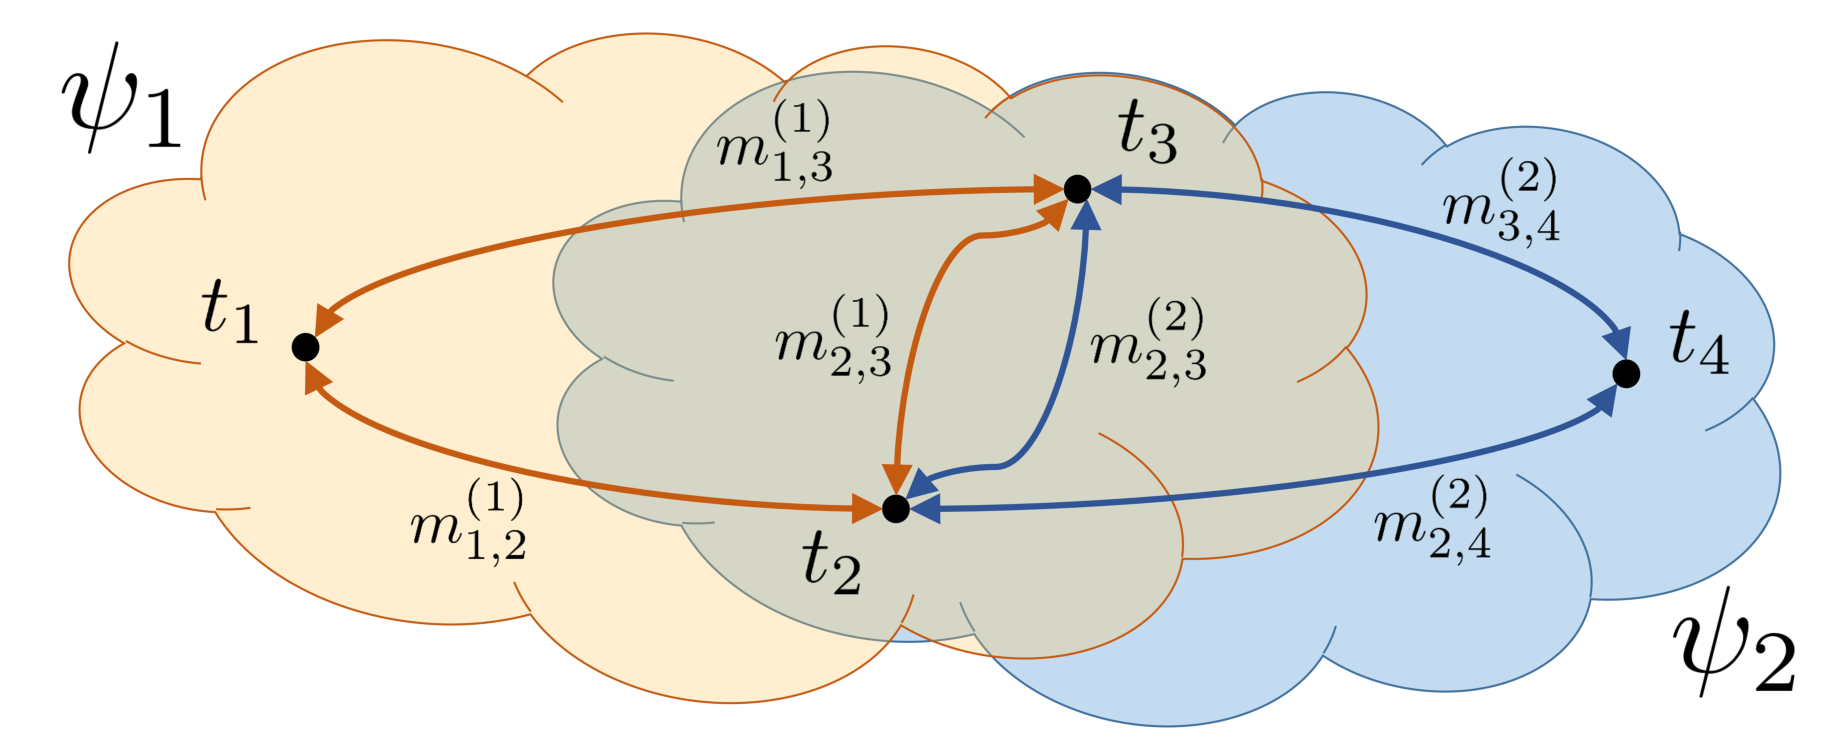
\includegraphics[width=0.9\textwidth]{img/DCSM/DCSM1}
        %\includegraphics[width=0.35\textwidth]{img/DCSM/duecontesti_relation_arrows.eps}
        \caption{A representation of the DCSM with the terms $t_1, ... t_4$ and the overlapping contexts $\psi_1, \psi_2$, where their semantic relationship is modeled by $m_{ij}^{(k)}$ with $i, j=1,...,4$ and $k=1,2$.  %\MAX{espandere la caption. cosa ci vuole dire l'immagine, casa indicano i simboli ?}
        }
    \label{fig:DCSMmodel}
\end{figure}

\subsection{The contextual semantic spaces}
Given a vocabulary $\mathcal{V}=\{t_1, ..., t_{T} \}$ of $T$ terms, we define a \textit{context} $\psi_k$ as a subset of $\mathcal{V}$ that represents a specific musical aspect. A descriptor $t_i$ is in the context $\psi_k$ if it \textit{has a semantics} within that context, i.e., if it is commonly used to describe the related musical aspect. We formalize this concept as 
\begin{equation}
\mathcal{V} \supset \psi_k = \{t_i \text{ has a semantics in } \psi_k \}.
\end{equation}
and we assume to model $K$ contexts $\psi_1, ..., \psi_K$.

In order to model the polysemy, the sets of contexts can generally have an overlap, therefore a term may belong to multiple contexts. 
As an example, Fig. \ref{fig:DCSMmodel} depicts a possible scenario with two contexts $\psi_1$ and $\psi_2$ and $4$ terms $t_1$, $t_2$, $t_3$, $t_4$. The terms $t_2$, $t_3$ belong to both the contexts.

We model the semantic relationship between terms by assigning a \textit{similarity score} $m_{ij}^{(k)}$ to each pair of descriptors $t_i, t_j$ in each context $\psi_k$. More formally: 
\begin{equation}
m_{ij}^{(k)} = m_{ji}^{(k)} \in \; [-1, 1] \; \forall \; t_i, \; t_j \; \in \; \mathcal{V}, \;  \forall \;  k  = 1, ..., K, 
\end{equation}
where $K$ is the number of contexts. 
Given a generic context $\psi_k$, negative values of $m_{ij}^{(k)}$ represent the degree of dissimilarity, down to $-1$, i.e., perfect antonymy, whereas positive values represents a degree of semantic similarity, up to $1$, i.e., the perfect synonymy.
%that the two terms have opposite meaning in the context $\psi_k$, down to the value $-1$ (antonymy); positive values express similar meaning, up to $1$ (synonymy). 
The $0$ value expresses the absence of a semantic relation between the two terms in the context $\psi_k$. This is also the case of one of the terms that does not have a semantics in $\psi_k$:
\begin{equation}
t_i \notin \psi_k \implies m_{ij}^{(k)}=m_{ji}^{(k)}=0  \;\forall \; j =1,..., T.
\end{equation} 
In the example in Fig. \ref{fig:DCSMmodel}, $t_2$ and $t_3$ have (generally different) similarity scores $m^{(1)}_{2,3}$ and $ m^{(2)}_{2,3}$, with respect to the two possible contexts $\psi_1$ and $\psi_2$ respectively. 
Instead, the terms $t_1$ and $t_4$ are not prone to potential ambiguities, since they have a semantic in a unique context: $m^{(1)}_{1,4}=m^{(2)}_{1,4}=0$.
%we display a simplified representation of our model, with $4$ terms and $2$ contexts, with $\psi_a=\{t_1, t_2, t_3\}$ and $\psi_b =\{t_2, t_3, t_4\}$. 

We collect a set of $K$ symmetric \textit{similarity matrices} $\mathbf{M}^{(k)} \in \mathbb{R}^{T \times T}$, which are composed by the elements $m^{(k)}_{ij}$. Such matrices will be used to enrich a music description and to disambiguate terms that exhibit polysemy in a query from user. 

\subsection{Music description and modeling of user query}
\label{subsec:DCSMquery}
Given a set $\mathcal{S}$ of $N$ musical items, we describe each one as a vector 
\begin{equation}
\mathbf{s}_i = \lbrack w_1,...,w_j,...,w_{T} \rbrack \T \;
\end{equation}
where $w_j \in [-1,1]$ expresses the relevance of the correspondent term $t_j$ to describe the musical item $s_i$. Negative values of $w_j$ express that the item $s_i$ could be described with an antonym of the term $t_j$.

%In a music search engine based on query by semantic description, 
Musical items are retrieved by means of a query $q$ that we model as a vector 
\begin{equation}
\mathbf{q} = \lbrack w_1,...,w_j,...,w_{T} \rbrack \T ,
\label{eq:DCSM:q}
\end{equation}
 with $w_j=\rho_j$ if the $j$-th term is in the query and 0 otherwise. The variable $\rho_j \in [-1, 1]$ expresses the desired intensity for the descriptor $t_j$. %General search systems allow the user to specify which descriptors will be considered in the results, but not which ones will be excluded. 
Negative values of $\rho_j$ express how much a descriptor is \textit{not} desired to be present in the retrieved items, whereas positive values represent how much it is. The $0$ value is the neutral weight and expresses that the correspondent term is not relevant for the query.

Music descriptions and queries may both exhibit missing weights. On one hand, classical approaches to music pieces annotation are based on manual annotation by users (e.g., social tagging \cite{lamere2009}) or by automatic annotation (\textit{autotagging} \cite{Zanoni2012}). This has the effect to produce description vectors $\mathbf{s}_i$ that may be weakly annotated, i.e., be annotated with only a subset of the terms in the vocabulary \cite{lamere2009, Miotto2012}. 
On the other hand, when composing a query, users are likely to use only few relevant terms, according to their typical vocabulary. The missing weights are represented with $w_j=0$, since it is not possible to distinguish them from the non-relevent weights. As an example, from a query asking for a \textit{calm} song, it is not possible to determine why the \textit{quiet} descriptor has not been used, whether this is due to the non-relevance of the quality \textit{quiet} for the query or due to a fortuitous user's choice of the term. 

Ambiguity is a further issue in music description and retrieval systems. A set of tags and a query, in fact, may use ambiguous descriptors that belong to different contexts.
We exploit the DCSM in order to produce full-labeled and not ambiguous description vectors $\mathbf{s}_i$ and queries $\mathbf{q}$ by an enrichment procedure.


\begin{figure}[tbp]
        \centering
         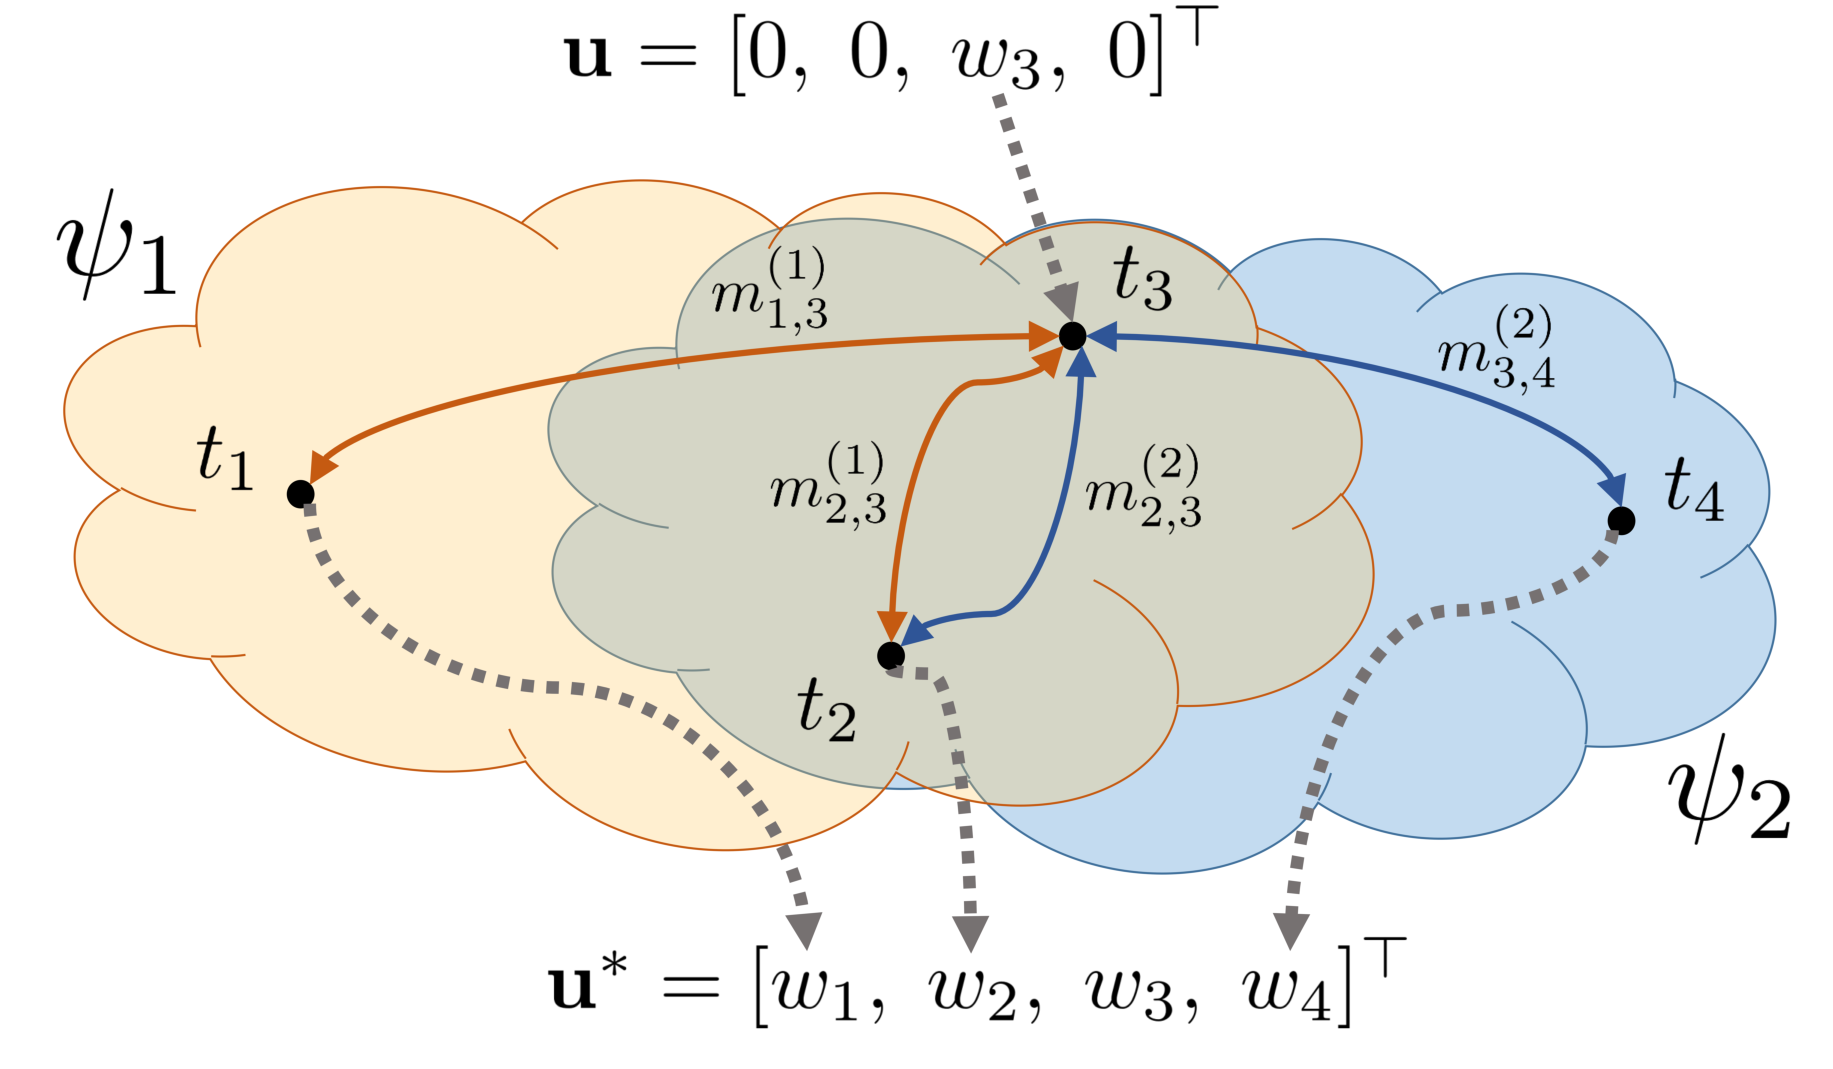
\includegraphics[width=0.9\textwidth]{img/DCSM/DCSM2}
        %\includegraphics[width=0.35\textwidth]{img/DCSM/duecontesti_relation_arrows_expand.eps}
        \caption{A representation of the semantic enrichment of a generic vector $\mathbf{u}$ with the DCSM by inferring the missing weigths $w_j=0$ from $ w_{3} \neq 0 $ and $m_{3,j}^{(k)}$. % \MAX{ESPANDERE}
        }
    \label{fig:DCSMexpand}
\end{figure}

\subsection{Exploiting the DCSM}
\label{subsec:DCSMenrichment}
In the following, we will use the generic notation $\mathbf{u} \in \mathbb{R}^T$ to indicate a generic vector of weights that can represent either a song description or a query. We aim at inferring the possibly missing weights ($w_j = 0$) by means of the present weights $w_i \neq0$ and the similarity scores $\mathbf{m}_{ij}^{(k)}$, in order to obtain an enriched vector $\mathbf{u}^*$. We can see the description as an overdetermined problem, where the equations, i.e. the set of similarities among the descriptors, are more than the unknown variables, i.e., the missing weights. An intuitive representation of this procedure is shown in Fig. \ref{fig:DCSMexpand}, where the missing weights $w_1=w_2=w_4=0$ are inferred by combining the present weight $w_3$ with the similarity scores for each context. Since $t_2$ and $t_3$ have two contexts in common, it is first needed to disambiguate the context. We address this ambiguity issue by weighting the contribution of the contexts $\psi_1$ and $\psi_2$ to $\mathbf{u}$.

We first define $\mathcal{W}^{(k)}=\{j: t_j \in \psi_k \land w_j \neq 0\}$ as the set of indices $j$ of the terms $t_j$ in the $k$-th context and whose weights are defined in $\mathbf{u}$. Afterwards, we define $ p(\psi_k | t_j) $ as the conditional probability that a term $t_j$ has a meaning in the context $\psi_k$. This probability is derived by the manual annotations of the terms, as described in Section \ref{sem_survey}. We compute the contribution of the context $\psi_k$ to $\mathbf{u}$ as a normalized sum of the contributions of all the terms for the $k$-th context:

\begin{equation}
p(\psi_k | \mathbf{u}) = \frac{ \sum_{j \in \mathcal{W}^{(k)} } p(\psi_k | t_j) }{\sum_{k =1 }^K \Big( \sum_{j \in \mathcal{W}^{(k)} } p(\psi_k | t_j) \Big)}.
\label{eq:prob_1}
\end{equation}

Finally, we derive the enriched vector $\mathbf{u}^*$ by weighting the sum of the contributions of the contexts to the vector:
\begin{equation}
\mathbf{u}^* = \sum_{k =1}^{K} p(\psi_k | \mathbf{u}) \mathbf{M}^{(k)} \mathbf{u}.
\end{equation}

The similarity matrices $\mathbf{M}^{(k)}$  help addressing the weak labeling issue by exploiting the similarity among descriptors. The issue of polysemy is addressed by the conditional probabilities $p(\psi_k | \mathbf{u})$, which weight the similarities through the contexts. Also in case of full-annotated description, we take advantage of the similarity matrices to regularize the description. 

% The semantic model we propose in this study allows to infer full-annotated description $\tilde{\mathbf{d}}$ exploiting the relation among terms within a context.
% %by applying the similarity matrices to the original item description $\mathbf{d}$, i.e., by means of the semantic relations of missing annotations ($w_i=0$) with present ones ($w_j \neq 0$). 
% Since the semantical relation among terms depends on the context, we compute the missing annotations as a weighted sum of the annotations in the description vector $\mathbf{d}$ multiplied to the similarity matrices $\mathbf{S}^{(k)}$ for each context $\psi_k$. The sum is weighted by the probability $ p(\psi_k | \mathbf{d})$ that a music item description $\mathbf{d}$ is referred to a certain context $\psi_k$:  %\MAX{Non è chiaro perché il vettore d deve appartenere ad un contesto.}
% \begin{equation}
% \tilde{\mathbf{d}} = \sum_{\psi_k \in \mathcal{C}} p(\psi_k | \mathbf{d}) \mathbf{S}^{(k)} \mathbf{d}.
% \end{equation}

% Given the set $\mathcal{D}^{(k)}=\{t_j \in \psi_k: w_j \neq 0\}$ of the terms $t_j$ that are in the context $\psi_k$ such that the correspondent weights are present in the description, we derive the probability $p(\psi_k | \mathbf{d}) $ as:
% \begin{equation}
% p(\psi_k | \mathbf{d}) = \frac{ \sum_{t_j \in \mathcal{D}^{(k)} } p(\psi_k | t_j) }{\sum_{\psi_k \in \mathcal{C} } \Big( \sum_{t_j \in \mathcal{D}^{(k)} } p(\psi_k | t_j) \Big)} ,
% \label{eq:prob_1}
% \end{equation}
% where $ p(\psi | t_j) $ is the probability of a term $t_j$ to be in the context $\psi_k$ and it is derived from the manual annotations of the terms, such as described in Section \ref{sem_survey}.



% Our approach applies the context similarity matrices also to the query vector $\mathbf{q}$ in order to enrich the request and make it independent on the user's vocabulary. We compute the enriched query as:
% \begin{equation}
% \tilde{\mathbf{q}} = \sum_{\psi_k \in \mathcal{C}} p(\psi_k | \mathbf{q}) \mathbf{S}^{(k)} \mathbf{q},
% \label{eq:tilde_query}
% \end{equation}
% where $p(\psi_k | \mathbf{q})$ is the probability of the context to be descriptive for the query and it is computed similarly to Equation \ref{eq:prob_1}.% and \ref{eq:prob_2}. 


\section{Implementation of the music search engine}
\label{sec:DCSMapplication}
%We developed a prototype of a music search engine application in order to validate our model.  
%A music search system receives as input a user query and returns music pieces that best fulfill to the request. 

%Our system is therefore composed by: the collection of the terms in the vocabulary $\mathcal{V}$, the definition of the contexts ${\psi \in \mathcal{C}}$ and the creation of similarity matrices $\mathbf{S}^\psi$; the annotation of music items $d$ in the terms vector space model with a description vector $\mathbf{d}$; the model of the user request $q$ as a query vector $\mathbf{q}$; the definition of a similarity function $\Xi$ that defines the degree of matching between the query $q$ and the music items $d_1, ..., d_N$. 


\begin{table}[tbp]
\caption{List of terms for each context cluster, obtained with the survey. Terms in bold italics present polysemy}
\label{tab:DCSMcontext}
\centering
\bgroup
\def\arraystretch{1.5}
\begin{tabular}{||p{.3\textwidth}|p{.6\textwidth}||}
\hline
\hline
Context & Descriptors\\
\hline
\hline
\bf{Perceived Emotion} & Aggressive, Angry, Annoyed, Anxious, Boring, Carefree, \textbf{\textit{Calm}}, Cheerful, Depressed, \textit{\textbf{Dark}}, 
Exciting, Fun, Frustrated, Funny, Happy, Joyful, Light, Nervous,\textit{\textbf{Quiet}}, \textbf{\textit{Relaxed}},  Sad, Serious, Sweet, Tender, Tense\\
\hline
\bf{Timbral Description} & Bright, Clean, \textit{\textbf{Dark}}, Hard, Harsh, Heavy, Rough, Smooth, Soft, Warm \\
\hline
\bf{Dynamics} & Dynamic, \textbf{\textit{Calm}}, Fast, Flowing, \textit{\textbf{Quiet}}, \textbf{\textit{Relaxed}}, Slow, Static, Stuttering\\
\hline
\hline
\end{tabular}
\egroup
\end{table}


\subsection{Setup of the semantic model}
\label{sem_survey}
In order to test the DCSM, we compose the vocabulary $\mathcal{V}$ of $T=40$ representative terms frequently used in music description applications (Table \ref{tab:DCSMcontext}). $\mathcal{V}$ contains descriptors from the ANEW dataset \cite{Bradley1999} and from those defined in  \cite{lesaffre2008} and used also in \cite{Buccoli2013}. We selected $K=3$ contexts that capture the following musical aspects: \textbf{Perceived Emotion} concerns the perceived mood of a song; \textbf{Timbre} refers to the sound characteristics of music; \textbf{Dynamics} is related to the dynamic characteristics (over loudness and tempo) of the music piece.

The definition of the meaning of terms and of the semantic similarity between terms is a popular problem in the literature \cite{Deerwester1990}. Dealing with thousand of terms makes a human annotation not affordable. In this study, we use a reduced vocabulary to tackle this issue. We collected semantic information through a two-stage survey.

In the first stage of the survey, a subset of randomly chosen terms from $\mathcal{V}$ was proposed to each participant, who was asked to assign each term to the context(s) in which it was deemed to have meaning. $135$ people participated to this first step and we collected at least $68$ annotations per term. We select only the term-context association with a high consensus, i.e., with a high ratio $r(t_i, \psi_k)$:
 \begin{equation}
t_i \in \psi_k \Longleftrightarrow   r(t_i, \psi_k) = \frac{N_{i}^{(k)}}{N_{i}}\geq 0.7,
 %r(t_i, \psi_k) = \frac{N_{i}^{(k)}}{N_{i}}\geq 0.7,
 \end{equation}
where $N_i$ is the number of people who annotated the $i$-th term and $N_i^{(k)}$ is the number of people who annotated it as belonging to the $k$-th context. We do not consider weak associations ($r(t_i,\psi_k)<0.7$) in order to build a model with a strong consensus on the semantics and make it robust to the users' bias.

Referring to the Eq. \ref{eq:prob_1}, we compute the term-context probability by normalizing these ratios, such that:
 \begin{equation}
 p(\psi_k | t_i) =  \frac{r(t_i, \psi_k)}{\sum_{k=1}^K r(t_i, \psi_k)}.
 \label{eq:prob_3}
 \end{equation}  

 The selected terms and the relative contexts are listed in Table \ref{tab:DCSMcontext}. As assumed, some terms have a meaning in more than one contexts (\textit{calm}, \textit{quiet}, \textit{relaxed}, etc.).

%
%\begin{figure}[t]
%\centering    
%\subfloat[Learned Features]{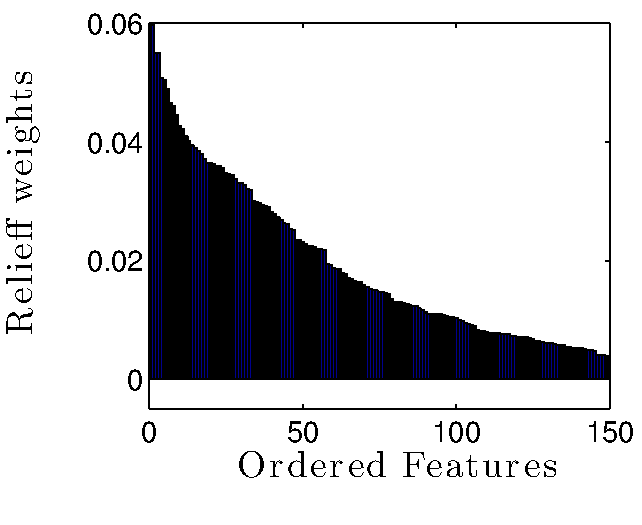
\includegraphics[width=.47\textwidth]{img/Bootleg/dbn_relieff_3}\label{fig:Bootleg:blabla}} \hfil
%\subfloat[Hand-Crafted Features]{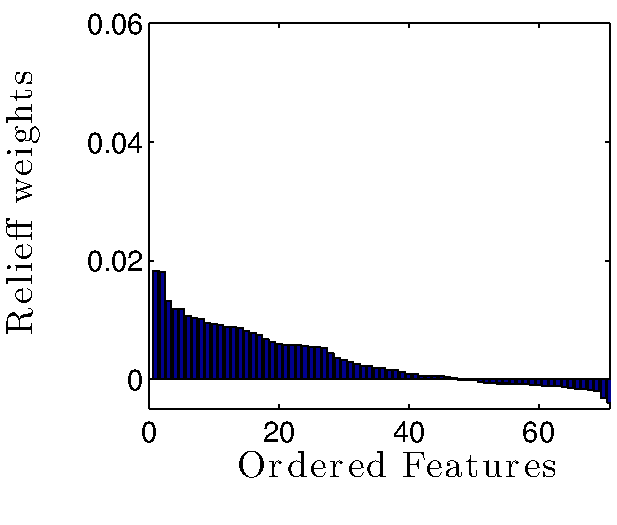
\includegraphics[width=.45\textwidth]{img/Bootleg/classic_relieff_3}\label{fig:Bootleg:lala}}
%\caption{Visualization of Relieff weights for learned (a) and hand-crafted (b) features. Notice how learned features' weights are strictly positive and assume higher values than hand-crafted features.}
%\label{fig:Bootleg:ueue}
%\end{figure}


\begin{figure}[tbp]
\centering    
\subfloat[Similarity scores between terms in the Perceived Emotion context]{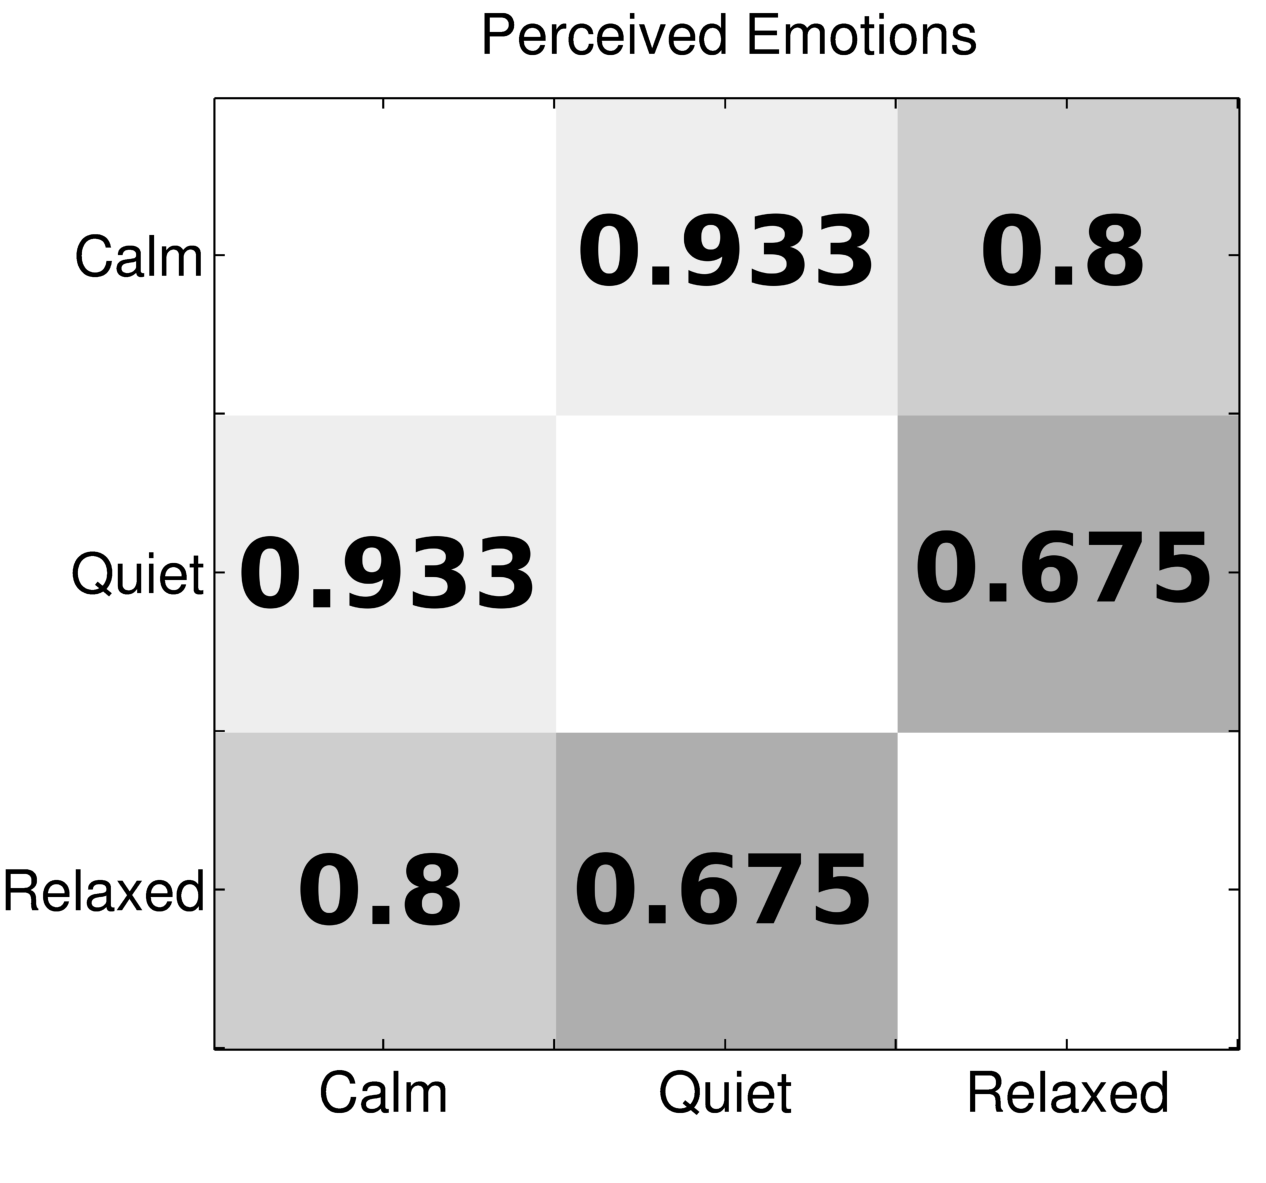
\includegraphics[width=.52\textwidth]{img/DCSM/mood_withValues}\label{fig:DCSM:mood}} \hfil
\subfloat[Similarity scores between terms in the Dynamics context]{\includegraphics[width=.433\textwidth]{img/DCSM/dyns_withValues}\label{fig:DCSM:dyn}}
\caption{Similarity scores between terms \textit{Calm}, \textit{Quiet}, \textit{Relaxed }in the \textit{Perceived Emotion} and \textit{Dynamics} contexts}
\label{fig:DCSM:similarity}
\end{figure}


In the second stage of the survey, each pair of terms in the same context was proposed to the testers, who were asked to annotate their semantic similarity for a given context, with a value ranging from $-1$ (antonyms) to $1$ (synonyms). $170$ testers were able to annotate each pair at least $3$ times. We observed similar annotation results among native English speaker and other participants for both parts of the survey, thus we assume that the results are not biased by the language knowledge of the testers.

In order to express the influence of the context in the similarity between terms, we show in Figure \ref{fig:DCSM:similarity} the similarity we obtained from annotations for the terms \textit{Calm}, \textit{Quiet} and \textit{Relaxed} in the two different contexts in which they have a meaning, i.e. the Perceived Mood (Fig. \ref{fig:DCSM:mood}) and (Fig. \ref{fig:DCSM:dyn}). We focus in particular on the pair of descriptors \textit{Quiet} and \textit{Relaxed}. In the context of Perceived Emotion, the annotations reveal a strong similarity among them, probably due to the fact that the two emotional states frequently occur together. In the context of Dynamics, however, the correlation is far lower and almost null. This is because when describing the Dynamics of the song as \textit{Relaxed}, we usually refer to a slow tempo, long notes and smooth transitions, while a song is often described as \textit{Quiet}  when it presents a low loudness. A \textit{Calm} song (in the Dynamics context) commonly summarizes the two aspects of a song, hence it presents a strong similarity with both terms.

\subsection{Description of music items}
\label{dataset}

In order to develop a real music search engine application, we use the public-available MsLite dataset \cite{Youngmoo2008}, which contains $N=240$ music excerpts annotated in the Valence-Arousal space. In JANAS the same dataset is annotated with non-emotional related descriptors. We used the non-emotional annotations by scaling their range ($[0- 10]$) to ours ($[-1, 1]$). We then compute the similarity between terms and songs as described in \cite{Buccoli2013}, using Bayesian probabilities, to obtain the emotional-related annotations.

The generic term $t$ is annotated in the ANEW dataset with the average and diagonal covariance matrix of the annotations for Valence and Arousal:
\begin{equation} 
\boldsymbol{\mu}_t=[\mu_V, \mu_A]\T ;
\end{equation}
\begin{equation} 
\boldsymbol{\Sigma}_t= 
%\begin{bmatrix}
\left[
\begin{aligned}[c c]
\sigma_V\quad & 0 \\
0 \quad & \sigma_A 
\end{aligned}
\right]
%\end{bmatrix}
\end{equation}
hence, the distribution of the semantics of the term in the VA space is modeled as a Normal distribution
\begin{equation}
t  \sim \mathcal{N}(\boldsymbol{\mu}_t,\boldsymbol{\Sigma}_t).
\end{equation} 

The songs from the dataset are also annotated in the VA space, and from the annotations we compute the mean and diagonal covariance matrix as the standard deviation of each component (Valence, Arousal), so that the generic song $s$ is modeled as 
\begin{equation}
s \sim \mathcal{N}(\boldsymbol{\mu}_s,\boldsymbol{\Sigma}_s).
\end{equation} 

We estimate how much the term $t$ is descriptive for the song $s$ by considering how much the latter belongs to the probability of the former, i.e.,
\begin{equation}
w_t = \text{exp} \left(-\frac{1}{2} (\boldsymbol{\mu}_t -\boldsymbol{\mu}_s)\T \boldsymbol{\Sigma}_t^{-1}  (\boldsymbol{\mu}_t -\boldsymbol{\mu}_s) \right).
\end{equation} 
We use the non-normalized distribution since we need the maximum value to be $1$, while the minimum value approaches $0$. Since the value is computed as a negative exponential difference, only songs whose average annotations is close enough to the mean of the term distribution receive positive annotations, so we are likely to obtain a weak labeling, where negative weights are not defined. We address the issues by leveraging the DCSM model.

We create the description vectors  $\mathbf{s}_1, ..., \mathbf{s}_N$ (Section \ref{subsec:DCSMquery}) by means of the aforementioned annotation procedure and we enrich them by means of the procedure explained in Section \ref{subsec:DCSMenrichment} to obtain $\mathbf{s}^*_1, ..., \mathbf{s}^*_N$.


\begin{table}[tbp]
\caption{Qualifiers and mean value weights from \cite{Rohrmann2003}, from the set $\mathcal{R}$, scaled to our model}
\label{tab:DCSMqualifiers}
%\begin{table}[h]%[tbp]
\centering
%\footnotesize
\bgroup
\def\arraystretch{1.5}
\begin{tabular}{||lcc||lcc||}
\hline
\hline
Qualifier & Weight & &  & Qualifier & Weight \\
\hline
\hline
a little & 0.5 & & & moderately & 0.6 \\ 
average & 0.7 & &   & not & -0.8  \\
completely & 1 & &  & not at all &  -1\\  
considerably & 0.9 & &  & partly & 0.7  \\
extremely & 1 & &  & quite & 0.6  \\
%fairly & 0.8 & & quite a bit & 0.5 \\ 
%fully & 1 & & rather & 0.7  \\
%hardly & 0.5 &   & slightly & 0.5  \\
%highly & 0.9 &  & somewhat & 0.7  \\
highly & 0.9 &  &  & slightly & 0.5  \\
%in-between & 0.7 &  & very & 0.8  \\
%mainly &  0.8 &   & very much & 0.9 \\
mainly &  0.8 &  &   & very & 0.8 \\
%medium & 0.7 & & & \\
\hline 
\hline
\end{tabular}
\egroup
\end{table}

\subsection{Retrieval of music items from user query}
Our music search system processes text-based queries using the natural language engine proposed in \cite{Buccoli2013}. This engine first processes the query with an automatic Part-Of-Speech (POS) processor, which identifies for each term its grammar role in the sentence, e.g., whether it is used as an adjective or a noun. The POS processor produces a tree structure that represent the organization of the sentence and the dependencies among terms, e.g., to which noun an adjective refers. In this way, we are able to extract not only the desired descriptors for the query, but also the desired intensity by means of \textit{qualifiers}, in order to fully exploit the properties of the semantic model.

We selected a set $\mathcal{R}$ of 14 common qualifiers by following the rating scale defined in \cite{Rohrmann2003} to allow the users to specify the desired intensity of each descriptor in the query. The set of qualifiers and their weights, scaled according to the semantics of our model, are listed in Table \ref{tab:DCSMqualifiers}. In the case no qualifier is specified, we assign the \textit{average} as the default value, i.e. $0.7$, instead of the maximum value $1$. We choose this value in order to avoid to mix the case where the desired intensity is not expressed with the case where the maximum of level intensity is required. Please also note that two negative-value qualifiers are defined, in order to express certain properties must not appear in the results of the query.

We model the query vector as $\mathbf{q}$ and enrich it to $\mathbf{q}^*$ as discussed in Sections \ref{subsec:DCSMquery} and \ref{subsec:DCSMenrichment}. Given a query $q$, and its enriched vector $\mathbf{q}^*$ and a generic enriched music item $\mathbf{s}_i^*$, we implement the musical items retrieval procedure by computing the score $\xi_{i q}$ by means of the cosine similarity:
\begin{equation}
\xi_{i q} = SC(\mathbf{s}_i^*,\mathbf{q}) 
		 = \frac{{\mathbf{q}^*}\T \mathbf{s}_i^*}{\|{\mathbf{q}^*} \| \|{\mathbf{s}_i^*} \|} \in [-1,1].
\end{equation}
We use the Cosine Similarity due to its range of values that include negative values when the angle between two vectors is wider than $\pi/2 $. In the DCSM model the $\pi/2 $ angle is interpreted as non-correlated items, while negative values identify opposite meaning.

The final retrieved items are returned by ranking the songs $s_1,...,s_N$ according to their scores. Due to the range of the Cosine Similarity, we only return songs whose score values are strictly positive.
\begin{table}[tbp]

\caption{Predefined queries for the subjective test, with the evaluating use case (UC)}
\label{tab:DCSM:queries}
\centering
\bgroup
\def\arraystretch{1.5}
\begin{tabular}{||l|p{.65\textwidth}|p{.15\textwidth}|p{.04\textwidth}||}
\hline
\hline
Id & Query & $\rho_i$ & UC \\
\hline
\hline
%1 & \textit{I want a highly relaxed and depressed song} & $(0.9, relaxed)$, $(0.7, depressed)$  & $P$ \\
%\hline
%2 & \textit{I would like to listen to a moderately angry track} & $(0.6, angry)$ & $OC$ \\
%\hline
%3 & \textit{I want a happy and quite exciting music piece} & $(0.7, happy)$, $(0.6, exciting)$ & $OC$ \\
%\hline
%4 & \textit{Give me a tender and considerably bright song} & $(0.7, tender)$. $(0.9, bright)$ & $ DC $\\
%\hline
%5 & \textit{Retrieve a little relaxed, moderately bright and static song} & $(0.5, relaxed)$, $(0.6, bright)$, $(0.7, static)$ & $ P$ \\
%\hline
%6 & \textit{I would like to listen to a dynamic and quite carefree track} & $(0.7, dynamic) $, $(0.6, carefree)$ & $ DC $ \\
%\hline
%7 & \textit{Please give me a hard, slightly aggressive and fast song} & $(0.5, aggressive)$, $(0.7, fast)$, $(0.7, hard)$ & $ DC $ \\
%\hline
%8 & \textit{Give me a little frustrated and partly calm song} & 
%$(0.5, frustrated)$, $(0.7, calm)$ & $P$ \\
%\hline
%9 & \textit{Give me a mainly dark, quite flowing and partly nervous track}  & $(0.8, dark)$, $(0.6, flowing)$, $(0.7, nervous)$ & $P $ \\
1 & \textit{I want a highly \textbf{relaxed} and \textbf{depressed} song} & $0.9, 0.7$  & $P$ \\
\hline
2 & \textit{I would like to listen to a moderately \textbf{angry} track} & $0.6 $ & $OC$ \\
\hline
3 & \textit{I want a \textbf{happy} and quite \textbf{exciting} music piece} & $0.7, 0.6$ & $OC$ \\
\hline
4 & \textit{Give me a \textbf{tender} and considerably \textbf{bright} song} & $0.7, 0.9 $ & $ DC $\\
\hline
5 & \textit{Retrieve a little \textbf{relaxed}, moderately \textbf{bright} and \textbf{static} song} & $0.5, 0.6, 0.7$ & $ P$ \\
\hline
6 & \textit{I would like to listen to a \textbf{dynamic} and quite \textbf{carefree} track} & $0.7, 0.6$ & $ DC $ \\
\hline
7 & \textit{Please give me a \textbf{hard}, slightly \textbf{aggressive} and \textbf{fast} song} & $0.7, 0.5, 0.7$ & $ DC $ \\
\hline
8 & \textit{Give me a little \textbf{frustrated} and partly \textbf{calm} song} & 
$0.5, 0.7$ & $P$ \\
\hline
9 & \textit{Give me a mainly \textbf{dark}, quite \textbf{flowing} and partly \textbf{nervous} track}  & $0.8, 0.6, 0.7$ & $P $ \\
\hline 
\hline
\end{tabular}
\egroup
\end{table}

\section{Model evaluation}
We compared our system with a LSA-based system \cite{Deerwester1990} and with the system JANAS proposed in \cite{Buccoli2013}. 

We build the LSA-based semantic model by exploiting the co-occurrences of song annotations and mapping the queries and the music description vectors in a $h$-dimensional reduced space. We build the matrix of representation $\mathbf{S}$ stacking all the non-expanded representations $\mathbf{s}_i$, and we compute a Singular Value Decomposition to compute a reduced dimensional space with $h=20$ as discussed in \ref{sec:HLFs:LSA}, where we mapped the songs' descriptions. The query $q$ is modeled as in Equation \ref{eq:DCSM:q}, and mapped in the h-dimensional LSA-based space, and the same cosine distance is used to compute the scores. 

JANAS, on the other hand, is based on a description model that uses two types of descriptors for music: emotional-related descriptors, mapped in the VA plane \cite{Russell1980} and non emotional-related descriptors, modeled as dimensional bipolar descriptors. The descriptors and the songs are modeled as normal probability distributions and their similarity is computed as a Bayesian posterior probability.

A common approach to validate information retrieval systems is to compare the retrieved items with a ground truth and evaluate the Precision, Recall and F-Measure of the retrieved items with respect to the correct ones. Unfortunately, building a ground truth is prohibitive for this scenario. %we are dealing with an average set of songs, and a $40$-dimensional continuous space of queries. Even 
Considering a set of $Q$ queries for evaluations, we would need at least $A$ annotations to estimate if each of the $N$ songs is relevant for each query, leading to $A*N*Q$ required annotations. As an example, a small set of $Q=20$ queries, with $A=3$ annotations each and $N=240$ songs would require 14,400 total annotations

For this reason, we evaluate the retrieval performance of the three systems by conducting a computationally and cognitively cheaper subjective test that we proposed to 34 subjects, who were mainly chosen among Master and Ph.D. students and Post-doc researchers of the Politecnico di Milano.
 
The subjects were asked to rate, in a 9-point Likert scale, the relevance to the queries of the songs retrieved by each semantic model. In order to avoid any bias, we conducted the test in a blind fashion, hence the results were presented to the participants without any indication on the generating model. The participants were not aware of which kind of study we were conducting, nor we mentioned the polysemy issue about the queries.
The subject were asked to evaluate the retrieved results for nine predefined queries and for a test where they could use free verbalizations. In the latter case, the testers were provided with the set of descriptors $\mathcal{V}$ and of qualifiers $\mathcal{R}$ defined in our model, and they were asked to use the systems with any query they want to test the system with.


The nine predefined queries are shown in Table \ref{tab:DCSM:queries}. Please note that the limited set of terms (Table \ref{tab:DCSMcontext}) and qualifiers (Table \ref{tab:DCSMqualifiers}) affect the formulation of queries, which sound poorly "natural". We will identify the queries with their id number as $Q1,...,Q9$. They have been chosen in order to test our systems with different use cases, also indicated in the table:
\begin{itemize}
\item in the \textbf{one context} ($OC$) use case  all the terms in the query belong to the same context ($Q2$, $Q3$);
\item the \textbf{different contexts} ($DC$) use case involves terms belonging to different contexts, but without any ambiguities, i.e., each term belongs to only one context ($Q4$, $Q6$, $Q7$);
\item the \textbf{polysemy} ($P$) use case, instead, also includes ambiguity in the query ($Q1$, $Q5$, $Q8$, $Q9$).
\end{itemize}

\begin{figure}[!tb]
        \centering
         \includegraphics[width=0.8\textwidth]{img/DCSM/boxplots_J}       
		\caption{Boxplots of the evaluations for the three semantic models. The number on the right indicates the average of annotations}
		\label{fig:DCSMresults}
\end{figure}

In Figure \ref{fig:DCSMresults} we show the boxplots of the annotations for the three use cases, as well as the overall annotations for all the queries and for the free evaluation of the system.

As for $OC$ use case, the DCSM performs similarly to LSA-based model, since it is not affected by the use of contexts, while the JANAS-based model, however, performs far worse. Both DCSM and LSA-based model receive low rates from some people; however it is interesting to notice that DCSM receive few low rates, which are therefore considered as outliers, while LSA-based model receive enough low rates to consider them in the distribution. The final averages of the LSA and DCSM systems are pretty close to each other and they are almost $7$, with the DCSM performing slightly better. We believe this similar behavior is due to the good similarity metrics inferred or defined in the two model. On the other side, JANAS does not perform well, since it attempts to retrieve the songs whose description is equally distant from the terms in the query, which might result in descriptions that do not match either of the terms.

In the $DC$ use case, the three models perform quite similarly, and there is not a clear prevalence of either of them. The DCSM receives annotations with a high variance, while annotations on LSA-based model are lower but constant. The results obtained by JANAS spans almost all the rates from 2 to 9. In this case, the DCSM expands the queries by considering similar terms in both contexts, while the LSA-based model retrieves any descriptor that might have co-occurred with those in the query. The latest approach is very common in the queries on the Internet, and we assume that the users are more used to it. On the other side, the DCSM has a novel approach which might be not appreciated by all the users, which is proven by the low rates we received. Nevertheless, the average of the results for DCSM is slightly higher than for LSA-based model. We could not understand the reason of such discordant annotations for the results achieved by JANAS.

The $P$ use case, as expected, exhibits the advantages in using the DCSM with respect to the other approaches and clearly highlights the bias introduced by ignoring the context in semantic description. In particular, the evaluations on LSA exhibit a notable drop of performance. This is clearly due to the lack of apriori information on the semantics of the descriptors, which cannot be retrieved by the simple analysis of the co-occurrence of them. On the other side, the DCSM performs as well as with the other use cases, proving to be able to effectively disambiguate user queries and it is, on average, rated even better than in the use case with Different Contexts. JANAS is valuable, but still exhibits far lower results. 

The average results over all the predefined queries  show again that our proposed approach is the best rated by the testers and JANAS is the worst. While the averages of the annotations of the DCSM and the LSA model are quite close, the distribution of such annotations shows a clear preference for our model. This is confirmed also by the Free Evaluation test, where the DCSM outperforms the other two approaches. We believe that the ability of DCSM to take into account the semantic contexts and the polysemy is the main reason of the highest results.  


\section{Final considerations}
\label{sec:DCSMconclusions}
In this Chapter we analyzed the problem of addressing the ambiguities and issues raised by the natural language in the formalization of a semantic domain. While in Section \ref{sec:HLFs:ANEW} we used some apriori information on the semantics to address the conceptual organization of emotional-related descriptors, in this Chapter the apriori information are used to design a semantic model that is able to consider descriptors from different contexts, and it is effectively applied to a real-word application scenario.

We formalize the semantic domain by means of a $T$-dimensional model, $T$ being  the number of descriptors, and we embed semantic information by defining possibly overlapping subset of terms to formalize the contexts and different degrees of similarity among descriptors for each musical context.  The semantic relations between descriptors, as well as their contexts membership, have been manually annotated through an online survey. 

We developed a prototype of a music search engine based on our model and we compared it %
with the model proposed in \cite{Buccoli2013} and with a LSA model based on co-occurrences \cite{Deerwester1990}. Subjective evaluations show that our model exhibits the best performance and it especially outperforms the others for complex queries containing terms that have different meanings in different contexts. 

